\mychapter{Image Processing}{Image Processing}{}
\label{chap:imgpros}

\mysection{Introduction}{Introduction}
\label{sec:imgintro}

\mysection{Pinhole Camera Model}{Pinhole Camera Model}
\label{sec:imgpinhole}

The ideal pinhole camera can be described as a plane and an optical center (a.k.a) the pinhole. Light will travel from an object throught the optical center.
And hit the plane at the opposite end of the optical center. The distance between the opitical center and the plane is called the focal length $f$.


\begin{figure}[H]
    \centering
    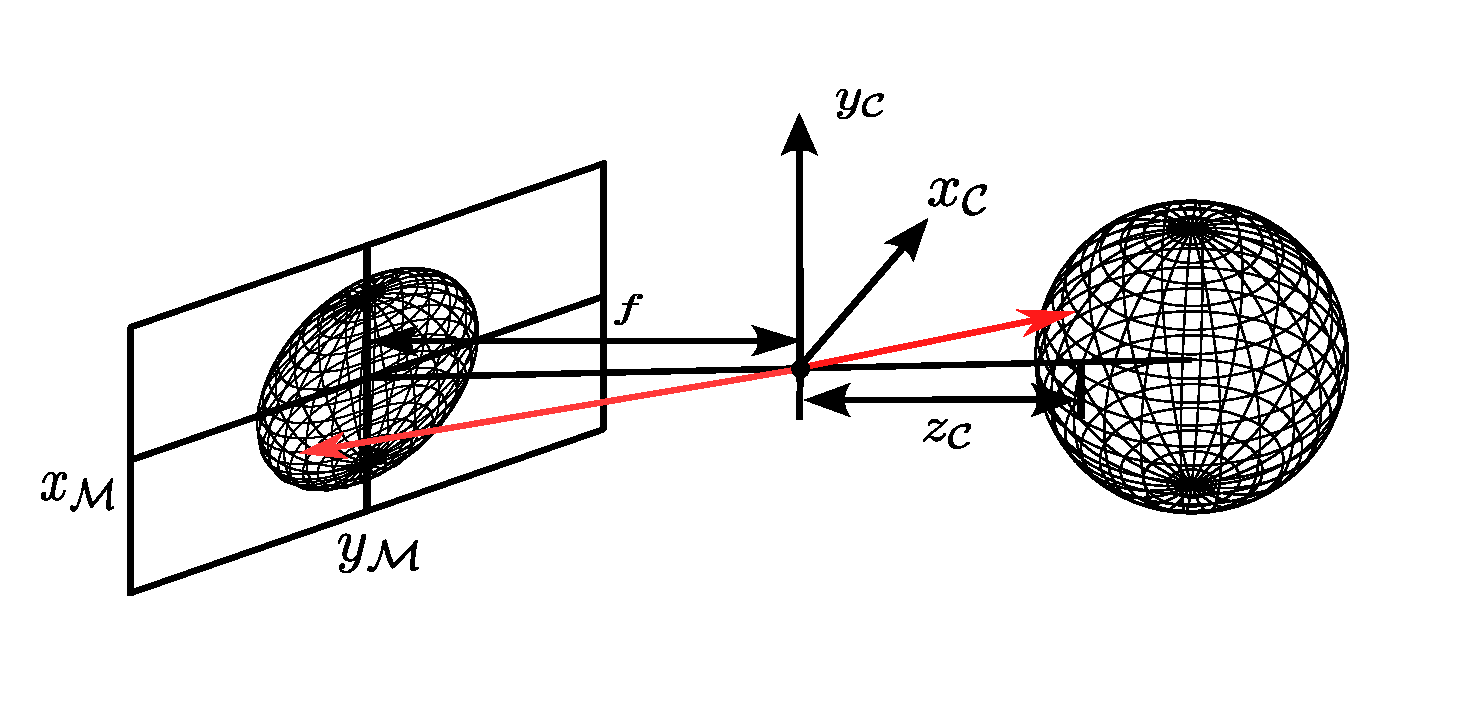
\includegraphics[width=1\linewidth]{figures/imageprocessing/Pinhole.pdf}
    \caption{PinHole Model}
    \label{fig}
\end{figure}


The equation for the pinhole camera model is the following.

\begin{equation}
\begin{bmatrix}
    x_\mathcal{M} \\
    y_\mathcal{M} \\
    1 
\end{bmatrix}
= \frac{-f}{z_\mathcal{C}}
\begin{bmatrix}
    x_\mathcal{C} \\
    y_\mathcal{C} \\
    z_\mathcal{C}
\end{bmatrix}
\end{equation}

As we can see in the figure this also causes the image tp flip.

Also images are measured with the x-axis going from right to left and the y-axis going from top to bottom so one more transformation needs to be done.

\begin{figure}[H]
    \centering
    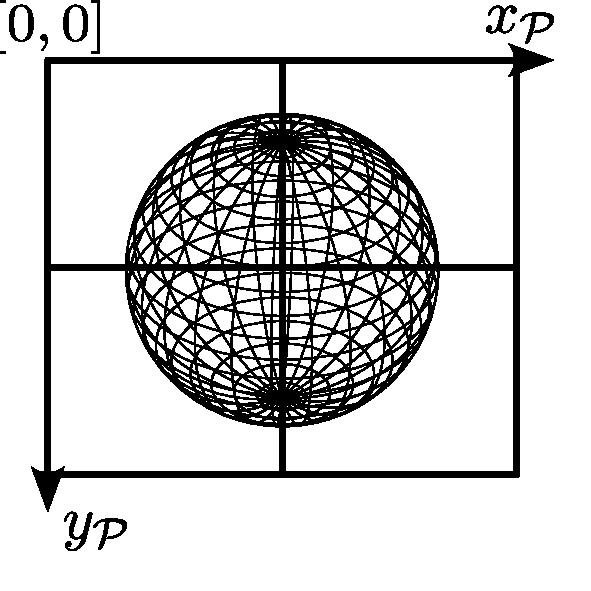
\includegraphics[width=0.5\linewidth]{figures/imageprocessing/ImagePlane.pdf}
    \caption{Image Plane}
    \label{fig4.2}
\end{figure}

\begin{equation}
\begin{bmatrix}
x_\mathcal{P} \\
y_\mathcal{P}
\end{bmatrix}
=
\begin{bmatrix}
    -x_\mathcal{M} + \frac{\text{ImgWidth}}{2} \\
    y_\mathcal{M} + \frac{\text{ImgHeight}}{2}
\end{bmatrix}
\end{equation}

\mysubsection{Camera Reference Frame}{Camera Reference Frame}

The camera refrence frame denoted by $\mathcal{C}$. In many Earth Observation missions the camera has its own reference frame defined relative to the Earth. Where the x-axis is
pointing directly to the Earth's surface indicatting the cameras roll axis, with the y-axis representing the pitch axis represents an angle ahead or behind of the orbit and the
z-axis representing the yaw axis.


\begin{figure}[H]
    \centering
    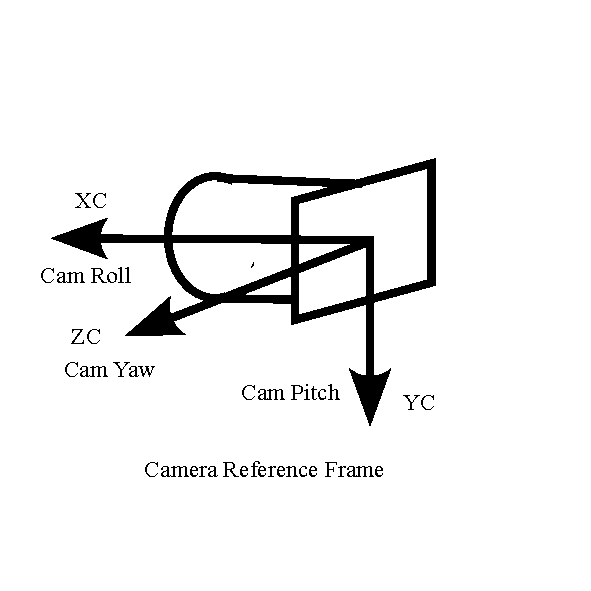
\includegraphics[width=0.4\textwidth]{figures/modelling/CRF.pdf}
    \caption{}
    \label{fig:CRF}
\end{figure}

\begin{equation}
    \mathbf{f}_{\mathcal{C}} = \mathbf{A}_{\mathcal{O}}^{\mathcal{C}}\times\mathbf{f}_{\mathcal{O}}
\end{equation}

\mysubsection{Image Reference Frame}{Image Reference Frame}

\begin{figure}[H]
    \centering
    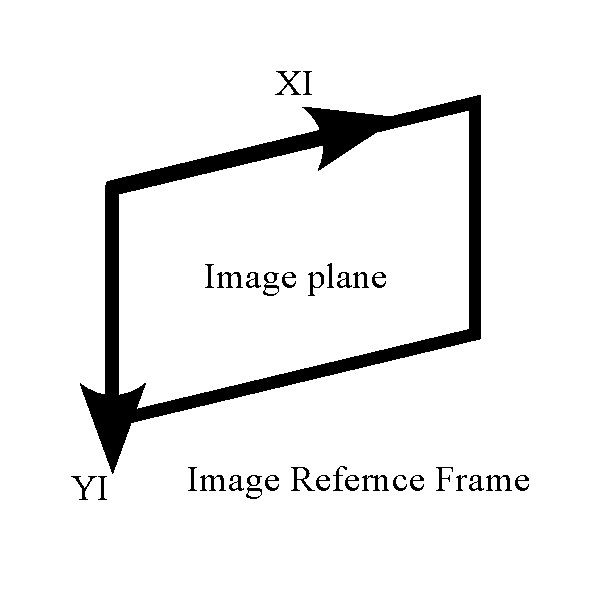
\includegraphics[width=0.4\textwidth]{figures/modelling/MRF.pdf}
    \caption{}
    \label{fig:MRF}
\end{figure}


%==================================================================================================================================================================================



\mysubsection{Intrinsic Camera Parameters}{Intrinsic Camera Parameters}

The projection plane coordinates of the projected point P can be converted into pixel baed measurements by expanding the projection matrix.

A horizontal and verticle scale factor $s_u$ and $s_v$ are defined as 


\begin{equation}
    s_u = \frac{\text{horizontal image resolution}}{\text{horizontal sensor size}}
\end{equation}

\begin{equation}
    s_v = \frac{\text{vertical image resolution}}{\text{vertical sensor size}}
\end{equation}

In the above equations, image resolution refers to the size, in pixels, of the resulting image captures by the modelled camera. Sensor size refers to the physical
size of the sensor, this means the scaling factor can be seen as having a unit of pixels per distance. These scaling factors can be incorporated with the focal length
of the camera to create factors $f_u$ and $f_v$ so that

\begin{equation}
    f_u = s_uf
\end{equation}

\begin{equation}
    f_v =s_vf
\end{equation}

Pixel based coordinates of the projected point $\mathbf{p}$ can be calculated with

\begin{equation}
    s
    \begin{bmatrix}
    u \\
    v \\
    1    
    \end{bmatrix}
    =
    \begin{bmatrix}
        f_u & 0 & 0 \\
        0 & f_v & 0 \\
        0 & 0 & 1
    \end{bmatrix}
    \begin{bmatrix}
        p_x \\ 
        p_y \\
        p_z
    \end{bmatrix}
\end{equation}

Where the s is the scaling factor. The Projection matrix in Equation ... can lastly be expanded with the offsets $o_u$ amd $o_v$ that ensure that the pixel-based
projection plane coordinates are in the lower-right quadrant, as in the convention with digital image. These offsets are defined as

\begin{equation}
    o_u = \frac{\text{horizontal image resolution}}{2}
\end{equation}

\begin{equation}
    o_v = \frac{\text{vertical image resolution}}{2}
\end{equation}

Pixel-based coordinated off the projected point $\mathbf{p}$ can be calculated in the typical convention with

\begin{equation}
    s
    \begin{bmatrix}
        u \\
        v \\
        1
    \end{bmatrix}
    =
    \begin{bmatrix}
    f_u & \alpha & o_u
    0 & f_v & o_v
    0 & 0 & 1
    \end{bmatrix}
    \begin{bmatrix}
        p_x \\
        p_y \\
        p_z
    \end{bmatrix}
\end{equation}

\begin{equation}
    = \mathbf{K}
    \begin{bmatrix}
    p_x \\
    p_y \\
    p_z
    \end{bmatrix}
\end{equation}

where $\mathbf{K}$ is known as the intrinsic matrix a skewing factor of $\alpha$ is added to adjust for skewing affects of the camera.

\mysubsection{Extrensic Camera Paramters}{Extrensic Camera Parameters}

In the equations it is assumed that the point being projected onto the image plane reference is defined in the camera reference frame. This
is not always the case and in certain circumstances the points that have to projected will have to be corrected the camera reference frame first.

An extrinsic camera matrix performs this conversion taks, it is made of a DCM $\mathbf{D}$ and translation vector $\mathbf{t}$ so that 

\begin{equation}
    [\mathbf{D}|\mathbf{t}] =
    \begin{bmatrix}
        d_{11} & d_{12} & d_{13} & t_1 \\
        d_{21} & d_{22} & d_{23} & t_2 \\
        d_{31} & d_{32} & d_{33} & t_3 \\
    \end{bmatrix}
\end{equation}

\begin{equation}
    s
    \begin{bmatrix}
        u \\
        v \\
        1
    \end{bmatrix}
    = \mathbf{K}[\mathbf{D}|\mathbf{t}]
    \begin{bmatrix}
        p_x \\
        p_y \\
        p_z \\
        1
    \end{bmatrix}
\end{equation}

\mysubsection{Back Projection}{Back Projection}

The intrinsic camera matrix discussed is typicall used to project 3D points in the camera referecne frame down to the 2D image plane reference frame. It can
also be used to project 2D coordinates on the image plane reference frame back into 3D space.

Assume the scaling factor $s$ is known or assumed.

The 3D vector can be reconstructed.

\begin{equation}
\mathbf{d} = s*\mathbf{K}^{-1}
\begin{bmatrix}
    u \\
    v \\
    1
\end{bmatrix}
\end{equation}


\mysection{Satellite Image Characteristics}{Satellite Image Characteristics}

\mysubsection{Ground Sample Distance}{Ground Sample Distance}
% Mathematical relationship

Ground Sampling Distance (GSD) is the real-world distance between the centers of two adjacent 
pixels measured on the ground in an image captured by a remote sensing system or satellite. It represents 
the spatial resolution of the imaging sensor and determines the level of detail visible in the image — smaller GSD 
values correspond to higher resolution, allowing finer features on the ground to be distinguished.

Where the mathematical relationship is

\begin{equation}
    GSD = \frac{\text{altitude} * \text{pixelsize} * \text{resolution}}{\text{focal length}}
\end{equation}


% Impact on feature detection accuracy
% Trade oofs with altitude and camera parameters


\mysubsection{Imaging Geometry}{Imaging Geometry}

% Nadir vs off-nadir imaging
% Field of view calculations

The field of view (FOV) of the satellite imager is calculated using the relationship between the camera's focal length, 
sensor dimensions, and pixel size. The vertical field of view is determined by the equation $\text{FOV}_v = 2 \times \arctan\left(\frac{I_y \times p_s}{2f}\right)$, 
where $I_y$ is the image height in pixels, $p_s$ is the pixel size, and $f$ is the focal length. For the horizontal field of view, the image width $I_x$ is 
substituted for $I_y$ in the calculation. This angular field of view defines the observable ground area from the satellite's orbital altitude, with the ground 
sample distance (GSD) providing the metric resolution per pixel according to $\text{GSD} = \frac{p_s \times h}{f}$, where $h$ is the altitude above the target 
surface. These geometric relationships are fundamental to the measurement model, as they establish the transformation between pixel coordinates in the image plane 
and the corresponding angular directions in the camera reference frame, enabling precise feature vector calculations for pose estimation.

% Ground coverage estimation
% Geometric distortions

\mysubsection{Lens Distortions}{Lens Distortions}

% Radial
% Tangential
% Abberations

\mysection{Feature Detection and Description}{Feature Detection and Description}

\mysubsection{Classical Feature Detectors}{Classical Feature Detectors}
% SIFT
\mysubsubsection{SIFT}{SIFT}

Scale-Invariant Feature Transform (SIFT) is a computer vision algorithm designed to detect and describe local features in images that remain 
stable under various transformations including scaling, rotation, and illumination changes. The algorithm operates in four main stages: scale-space extrema 
detection using Difference of Gaussians (DoG), keypoint localization through sub-pixel refinement, orientation assignment based on local gradient histograms, 
and descriptor generation using a 128-dimensional feature vector.

The scale-space representation is constructed by convolving the input image $I(x,y)$ with Gaussian kernels of increasing standard deviation:
\begin{equation}
L(x,y,\sigma) = G(x,y,\sigma) * I(x,y)
\end{equation}
where $G(x,y,\sigma) = \frac{1}{2\pi\sigma^2}e^{-(x^2+y^2)/2\sigma^2}$ is the Gaussian kernel. The DoG function approximates the Laplacian of Gaussian for 
efficient keypoint detection:
\begin{equation}
D(x,y,\sigma) = L(x,y,k\sigma) - L(x,y,\sigma)
\end{equation}
where $k$ is a constant multiplicative factor between adjacent scales.

For each detected keypoint, the dominant orientation is determined by computing the gradient magnitude and direction:
\begin{align}
m(x,y) &= \sqrt{[L(x+1,y) - L(x-1,y)]^2 + [L(x,y+1) - L(x,y-1)]^2} \\
\theta(x,y) &= \arctan\left(\frac{L(x,y+1) - L(x,y-1)}{L(x+1,y) - L(x-1,y)}\right)
\end{align}

The descriptor is constructed by sampling gradients in a 16×16 pixel neighborhood around the keypoint, subdivided into 4×4 blocks with 
8-bin orientation histograms, resulting in a 128-dimensional feature vector ($4 \times 4 \times 8 = 128$). Each descriptor element is weighted by 
the gradient magnitude and a Gaussian window centered at the keypoint. The resulting 128-dimensional descriptor provides robust matching capabilities 
across different viewing conditions, making SIFT particularly suitable for satellite imagery where features must be reliably detected despite changes in lighting, 
seasonal variations, and slight geometric distortions. However, the computational complexity of SIFT can be limiting for real-time applications, requiring careful 
consideration of the trade-off between feature quality and processing speed in resource-constrained satellite systems.

% SURF
\mysubsubsection{SURF}{SURF}

Speeded-Up Robust Features (SURF) is a computer vision algorithm developed as a faster alternative to SIFT while maintaining comparable performance 
in feature detection and description. SURF achieves computational efficiency through the use of integral images and approximations of the Laplacian of 
Gaussian operator, making it particularly suitable for real-time applications in resource-constrained satellite systems.

The algorithm utilizes integral images $I_{\Sigma}(x,y)$ to enable rapid computation of rectangular area sums:
\begin{equation}
I_{\Sigma}(x,y) = \sum_{i=0}^{i \leq x} \sum_{j=0}^{j \leq y} I(i,j)
\end{equation}
where $I(i,j)$ represents the intensity at pixel $(i,j)$. This allows any rectangular sum to be computed in constant time using only four array references.

SURF approximates the Laplacian of Gaussian using box filters that can be evaluated efficiently with integral images. The determinant of the Hessian matrix is used for keypoint detection:
\begin{equation}
\text{Det}(\mathbf{H}) = D_{xx}D_{yy} - (0.9D_{xy})^2
\end{equation}
where $D_{xx}$, $D_{yy}$, and $D_{xy}$ are the convolution responses of the image with the second-order Gaussian derivatives, approximated using box filters. The factor 0.9 is an empirical weight to balance the expression.

For orientation assignment, SURF computes Haar wavelet responses in the $x$ and $y$ directions within a circular neighborhood:
\begin{align}
d_x &= \text{Haar}_x * I(x,y) \\
d_y &= \text{Haar}_y * I(x,y)
\end{align}
The dominant orientation is determined by summing all responses within a sliding window of $\frac{\pi}{3}$ radians.

The SURF descriptor is typically 64-dimensional (compared to SIFT's 128), constructed by dividing a 20×20 pixel region around the keypoint into 4×4 sub-regions. 
For each sub-region, the wavelet responses are summed to create a 4-dimensional descriptor vector $\mathbf{v} = [\sum d_x, \sum d_y, \sum |d_x|, \sum |d_y|]$. 
This results in a $4 \times 4 \times 4 = 64$-dimensional descriptor that provides robust matching while requiring significantly less computational resources 
than SIFT, making it advantageous for satellite pose estimation applications where processing efficiency is critical.

% ORB
\mysubsubsection{ORB}{ORB}

Oriented FAST and Rotated BRIEF (ORB) is a binary feature descriptor that combines the FAST keypoint detector with the BRIEF descriptor, 
enhanced with orientation compensation to achieve rotation invariance. ORB is designed for real-time applications and provides significant computational 
advantages over SIFT and SURF, making it particularly suitable for resource-constrained satellite systems where processing efficiency is paramount.

The FAST (Features from Accelerated Segment Test) detector identifies keypoints by examining the intensity values of 16 pixels arranged in a circle around 
a candidate point $p$. A pixel $p$ is classified as a corner if there exists a set of $n$ contiguous pixels in the circle that are all brighter than $I_p + t$ or 
all darker than $I_p - t$, where $I_p$ is the intensity of pixel $p$ and $t$ is a threshold:
\begin{equation}
\text{FAST}(p) = \begin{cases}
1 & \text{if } \exists \text{ arc of length } n \text{ such that } \forall x \in \text{arc}: |I_x - I_p| > t \\
0 & \text{otherwise}
\end{cases}
\end{equation}

To achieve rotation invariance, ORB computes the intensity centroid to determine keypoint orientation. The moments of a patch are calculated as:
\begin{align}
m_{pq} &= \sum_{x,y} x^p y^q I(x,y) \\
\text{Centroid: } \mathbf{C} &= \left(\frac{m_{10}}{m_{00}}, \frac{m_{01}}{m_{00}}\right)
\end{align}
The orientation angle is then determined by:
\begin{equation}
\theta = \arctan\left(\frac{m_{01}}{m_{10}}\right)
\end{equation}

The BRIEF descriptor is modified to create rBRIEF (rotated BRIEF) by applying a rotation matrix to the sampling pattern. For a set of $n$ binary tests, 
each test $\tau$ compares the intensities of two pixels:
\begin{equation}
\tau(p; x, y) = \begin{cases}
1 & \text{if } p(x) < p(y) \\
0 & \text{otherwise}
\end{cases}
\end{equation}
The rotated sampling pattern is computed as:
\begin{equation}
\mathbf{S}_{\theta} = \mathbf{R}_{\theta} \mathbf{S}
\end{equation}
where $\mathbf{R}_{\theta}$ is the rotation matrix and $\mathbf{S}$ is the original sampling pattern.

The final ORB descriptor is a 256-bit binary string computed by applying the rotated BRIEF tests. This binary representation 
enables extremely fast matching using the Hamming distance, computed as:
\begin{equation}
d_H(\mathbf{a}, \mathbf{b}) = \sum_{i=1}^{n} a_i \oplus b_i
\end{equation}
where $\oplus$ denotes the XOR operation. The computational efficiency and low memory requirements of ORB make it ideal for satellite 
pose estimation applications where real-time performance and limited computational resources are critical constraints.


\mysubsubsection{Comparison}{Comparison}

% \mysubsection{Feature Description}{Feature Description}
% \label{sec:featuredescription}

% Local feature descriptors play a crucial role in satellite pose estimation by providing robust representations of image features 
% that can be matched across different viewing conditions. These descriptors encode the local appearance of image regions around detected 
% keypoints, creating distinctive signatures that enable reliable correspondence matching between images captured at different times, orientations, and lighting conditions.

% \mysubsubsection{Invariance Properties}{Invariance Properties}
% \label{sec:invarianceproperties}

% The effectiveness of feature descriptors in satellite applications depends critically on their invariance properties. Scale invariance ensures 
% that features remain detectable as the satellite altitude changes or when using different zoom levels. This is particularly important for Earth 
% observation satellites that may operate at varying altitudes or employ different imaging modes. Rotation invariance is essential for satellites 
% that experience attitude changes, as the same ground features must be recognizable regardless of the satellite's orientation relative to the Earth's surface.

% Illumination invariance addresses the challenge of varying lighting conditions caused by solar angle changes, seasonal variations, and atmospheric 
% effects. For satellite imagery, this property is vital as the same geographic features may be observed under drastically different illumination conditions 
% throughout the orbital period. Affine invariance provides robustness against perspective distortions that occur when observing the same ground features from 
% slightly different viewpoints, which is common in satellite imaging due to orbital mechanics and attitude variations.

% \mysubsubsection{Descriptor Matching Strategies}{Descriptor Matching Strategies}
% \label{sec:descriptormatching}

% Feature matching in satellite pose estimation typically employs distance-based similarity measures to establish correspondences between descriptors. 
% For floating-point descriptors like SIFT and SURF, the Euclidean distance provides a natural similarity metric:
% \begin{equation}
% d_E(\mathbf{f}_1, \mathbf{f}_2) = \sqrt{\sum_{i=1}^{n} (f_{1i} - f_{2i})^2}
% \end{equation}
% where $\mathbf{f}_1$ and $\mathbf{f}_2$ are $n$-dimensional descriptor vectors.

% For binary descriptors like ORB, the Hamming distance offers computational efficiency:
% \begin{equation}
% d_H(\mathbf{b}_1, \mathbf{b}_2) = \sum_{i=1}^{n} b_{1i} \oplus b_{2i}
% \end{equation}
% where $\oplus$ represents the XOR operation.

% The nearest neighbor matching strategy identifies the closest descriptor in the database, while the ratio test introduced by Lowe provides 
% additional robustness by comparing the distances to the first and second nearest neighbors:
% \begin{equation}
% \text{Ratio test: } \frac{d_1}{d_2} < \tau
% \end{equation}
% where $d_1$ and $d_2$ are the distances to the first and second nearest neighbors, respectively, and $\tau$ is a threshold typically set to 0.8.

% \mysubsubsection{Robustness to Viewpoint Changes}{Robustness to Viewpoint Changes}
% \label{sec:viewpointrobustness}

% Satellite pose estimation requires descriptors that maintain distinctiveness across moderate viewpoint changes. The challenge arises from the 
% fact that satellites observe the Earth from different positions along their orbital path, creating subtle but significant changes in the appearance 
% of ground features. Viewpoint invariance is typically achieved through normalization techniques that account for local geometric transformations.

% SIFT addresses viewpoint changes through its multi-scale pyramid representation and gradient-based orientation assignment, which provides robustness 
% to viewpoint variations up to approximately 30 degrees. SURF employs similar strategies but with computational optimizations, while ORB relies on the 
% intensity centroid method for orientation normalization.

% For satellite applications, additional robustness can be achieved through descriptor pooling techniques, where multiple descriptors from the same feature 
% are combined to create a more stable representation. Geometric verification using methods such as RANSAC (Random Sample Consensus) helps eliminate false matches 
% that may arise from descriptor ambiguities:
% \begin{equation}
% \mathbf{H} = \arg\min_{\mathbf{H}} \sum_{i=1}^{n} \rho(||\mathbf{p}_i' - \mathbf{H}\mathbf{p}_i||)
% \end{equation}
% where $\mathbf{H}$ is the homography matrix, $\mathbf{p}_i$ and $\mathbf{p}_i'$ are corresponding points, and $\rho$ is a robust cost function.

% The combination of invariant descriptors and robust matching strategies forms the foundation for reliable feature tracking in satellite pose estimation 
% systems, enabling accurate determination of spacecraft position and attitude through visual odometry and simultaneous localization and mapping (SLAM) techniques.

% \mysubsection{Feature Quality Assessment}{Feature Quality Assessment}


\mysection{Measurement Extraction}{Measurement Extraction}
\label{sec:imgmesurement}

\mysubsection{Image Generation}{Image Generation}

\mysubsubsection{Rendering the Earth}{Rendering the Earth}

To create an image

Fisrt a High resolution image is sticth in QGIS, a type fo Geographic information system, used to open an edit geolocated images.
Images a downloaded from the copernicus with a GSD of 15 m.

\textcolor{blue}{Insert Image of Paris}
\textcolor{blue}{Inert Image of Pyramids}
\textcolor{blue}{Insert Image of Hawaii Volcano}

After an high resolution image is sitched. It is rasterised.
This rasterised image with all its goelocation data is then projected onto a WGS84 ellipsoid.

\begin{figure}[H]
    \centering
    
\includegraphics[width=0.5\linewidth]{figures/imageprocessing/HighResImage.png}
    \caption{High Resolution Image projected on Ellipsoid}
    \label{}
\end{figure}

The Low resolution Earth in the Backgorund is used as a place holder to test results

\mysubsection{Earth Tracker Algorithm}{Earth Tracker Algorithm}

The Earth Tracker works on the same principle as Back projection.

\textbf{Step 1: Translate pixels to optical center}

The second step involes translating the pixel cooridnates to the optical center as the origin. This transformation accounts for the camera's principle point
offset, where $I_x$ and $I_y$ represent width and height, repsectivly. The resulting coordinate vector $\mathbf{f}_{\mathcal{M/S}}$ represents position Relative
to the camera boresight.

\begin{equation}
    \mathbf{f}_{\mathbf{M/S}} = 
    \begin{bmatrix}
        f_\mathcal{M} - \frac{I_x}{2} \\
        f_\mathcal{M} - \frac{I_y}{2}
    \end{bmatrix}
    \text{(Pixels)}
\end{equation}

\begin{figure}[H]
    \centering
    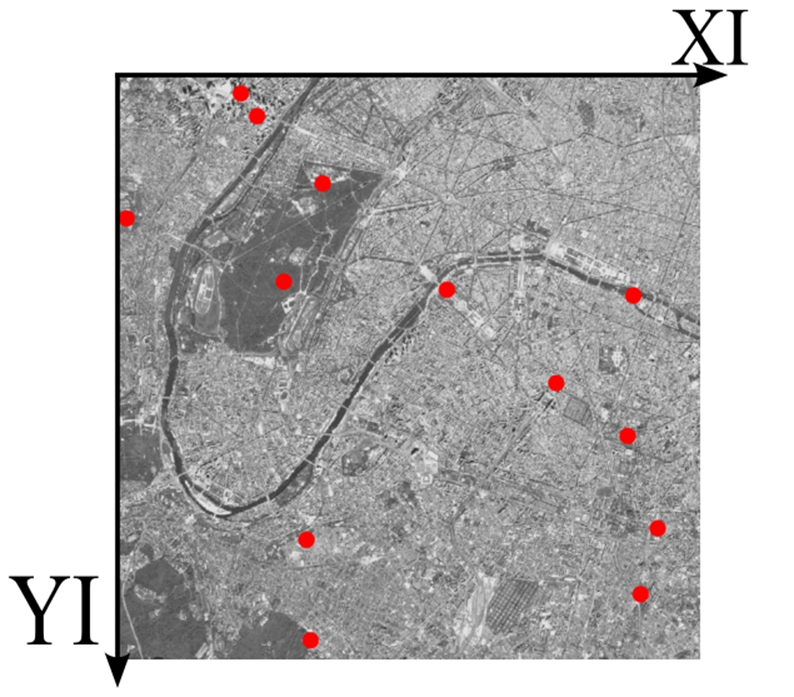
\includegraphics[width=0.5\linewidth]{figures/imageprocessing/IMG1.png}
    \caption{Origin Correction}
    \label{}
\end{figure}

\begin{figure}[H]
    \centering
    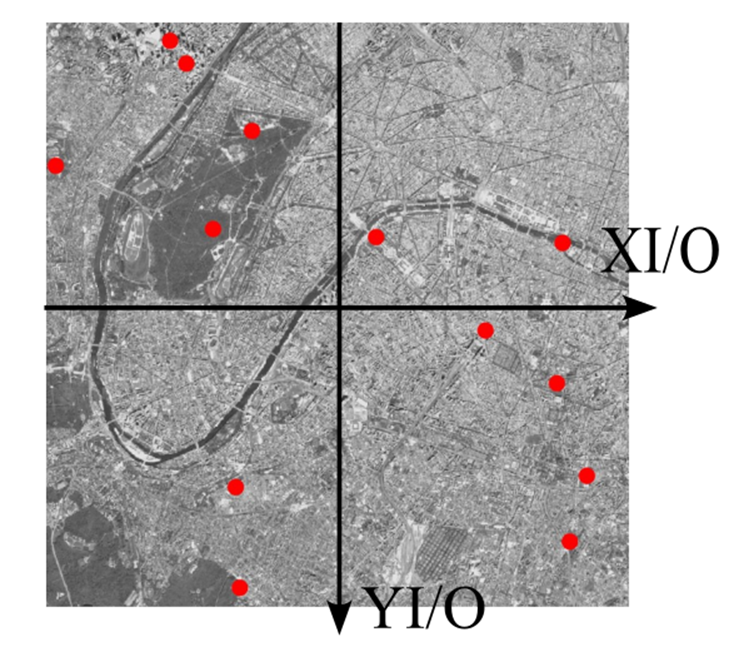
\includegraphics[width=0.5\linewidth]{figures/imageprocessing/IMG2.png}
    \caption{Origin Correction 2}
    \label{}
\end{figure}

\textbf{Step 2: Three-Dimentional Ray Vector Construction}

This step transform the 2 dimensional pixel coordinates into the three-dimensional direction vector in the camera frame. The vector $\mathbf{f}_\mathcal{M/F}$ represents
the feqture direction relative to the camera focal point, where the z-component is dtermined by the effective focal lenght in pixels

\begin{equation}
    \mathbf{f}_\mathcal{M/F} = 
    \begin{bmatrix}
        f_{\mathcal{M/S_x}} \\
        f_{\mathcal{M/S_y}} \\
        \frac{fl}{ps}
    \end{bmatrix}
\end{equation}

\textbf{Step 3: Scale dorection vector}

The 3rd step performs a cordinate transformation to orient the feature vector in the appropriate referecne direction. This operation inverts and scales the vector so that it
is correct in the camera reference frame

The sacling used is the assumed GSD

\begin{equation}
    \mathbf{f} = GSD \times \mathbf{f}
\end{equation}

\mysubsection{Geolocation Process}{Geolocation Process}

For the geolocation.

\textbf{Step 1: Chip Image}

\textbf{Step 2: Chip features}

\textbf{Step 3: Use SIFT for feauture matching}

\textbf{Step 4: Add geolocation}


\mysubsection{Practical Considerations}{Practical Considerations}

\mysubsubsection{Number of Valid Feature}{Number of Valid Features}


\mysubsection{Conslusion}{Conclusion}


